\subsection{Chaves e relacionamentos}

A Tabela \ref{tab:relacionamentos} consolida as chaves estrangeiras do modelo, com a cardinalidade e a obrigatoriedade de cada liga\c{c}\~ao.

\begin{table*}[!t]
\caption{Chaves e relacionamentos}
\label{tab:relacionamentos}
\centering
\scriptsize
\setlength{\tabcolsep}{2.5pt}
\begin{tabular}{|L{2.5cm}|L{2.9cm}|L{2.0cm}|L{2.1cm}|C{1.3cm}|C{1.5cm}|L{3.6cm}|}
\hline
\textbf{Tabela origem} & \textbf{Campo origem} & \textbf{Tabela destino} & \textbf{Campo destino} & \textbf{Cardina\-lidade} & \textbf{Obrigat\'orio?} & \textbf{Observa\c{c}\~oes} \\
\hline
\texttt{veiculo} & \texttt{id\_categoria} & \texttt{categoria} & \texttt{id\_categoria} & 1:N & Sim & Uma categoria classifica v\'arios ve\'iculos \\
\hline
\texttt{veiculo} & \texttt{id\_filial} & \texttt{filial} & \texttt{id\_filial} & 1:N & Sim & Filial de lota\c{c}\~ao do ve\'iculo \\
\hline
\texttt{documento\_veiculo} & \texttt{id\_veiculo} & \texttt{veiculo} & \texttt{id\_veiculo} & 1:1 & Sim & A PK \'e a pr\'opria FK, o que limita o relacionamento a um registro \\
\hline
\texttt{locacao} & \texttt{id\_cliente} & \texttt{cliente} & \texttt{id\_cliente} & 1:N & Sim & Um cliente realiza v\'arias loca\c{c}\~oes \\
\hline
\texttt{locacao} & \texttt{id\_veiculo} & \texttt{veiculo} & \texttt{id\_veiculo} & 1:N & Sim & Um ve\'iculo \'e alugado v\'arias vezes \\
\hline
\texttt{locacao} & \texttt{id\_filial\_retirada} & \texttt{filial} & \texttt{id\_filial} & 1:N & Sim & Filial onde o ve\'iculo foi retirado \\
\hline
\texttt{locacao} & \texttt{id\_filial\_devolucao} & \texttt{filial} & \texttt{id\_filial} & 1:N & Sim & Pode ser diferente da filial de retirada \\
\hline
\texttt{manutencao} & \texttt{id\_veiculo} & \texttt{veiculo} & \texttt{id\_veiculo} & 1:N & Sim & Um ve\'iculo sofre v\'arias manuten\c{c}\~oes \\
\hline
\texttt{cliente} & (via \texttt{locacao}) & \texttt{veiculo} & (via \texttt{locacao}) & N:N & N\~ao & Relacionamento conceitual resolvido pela tabela associativa \texttt{locacao} \\
\hline
\end{tabular}
\end{table*}

\subsection{Dom\'inios e valores controlados}

Os campos com conjunto fechado de valores est\~ao na Tabela \ref{tab:dominios}. A valida\c{c}\~ao \'e feita por restri\c{c}\~ao \texttt{CHECK} no MySQL 8.

\begin{table*}[!t]
\caption{Dom\'inios e valores controlados}
\label{tab:dominios}
\centering
\scriptsize
\setlength{\tabcolsep}{2.5pt}
\begin{tabular}{|L{3.4cm}|L{2.6cm}|L{7.4cm}|C{1.4cm}|}
\hline
\textbf{Campo} & \textbf{Valor} & \textbf{Descri\c{c}\~ao} & \textbf{Ativo?} \\
\hline
\multirow{3}{*}{\texttt{cliente.status}} & ATIVO & Cliente apto a locar & Sim \\
 & INATIVO & Cadastro sem movimenta\c{c}\~ao & Sim \\
 & BLOQUEADO & Impedido de locar & Sim \\
\hline
\multirow{4}{*}{\texttt{veiculo.status}} & DISPONIVEL & Livre para loca\c{c}\~ao & Sim \\
 & LOCADO & Em poder de um cliente & Sim \\
 & MANUTENCAO & Em oficina & Sim \\
 & INATIVO & Fora da frota & Sim \\
\hline
\multirow{5}{*}{\texttt{veiculo.combustivel}} & FLEX & Etanol e gasolina & Sim \\
 & GASOLINA & Somente gasolina & Sim \\
 & DIESEL & Somente diesel & Sim \\
 & ELETRICO & Motor el\'etrico & Sim \\
 & HIBRIDO & Combust\~ao e el\'etrico & Sim \\
\hline
\multirow{3}{*}{\texttt{locacao.status}} & ABERTA & Ve\'iculo ainda n\~ao devolvido & Sim \\
 & FINALIZADA & Devolu\c{c}\~ao registrada & Sim \\
 & CANCELADA & Contrato desfeito & Sim \\
\hline
\multirow{3}{*}{\texttt{manutencao.tipo}} & PREVENTIVA & Programada por km ou prazo & Sim \\
 & CORRETIVA & Reparo de falha & Sim \\
 & REVISAO & Revis\~ao de garantia & Sim \\
\hline
\multirow{6}{*}{\texttt{cliente.cat\_cnh}} & A & Motocicletas & Sim \\
 & B & Autom\'oveis & Sim \\
 & AB & Ambas & Sim \\
 & C, D, E & Cargas e passageiros & Sim \\
\hline
\end{tabular}
\end{table*}

\subsection{\'Indices}

Al\'em dos \'indices criados automaticamente pelas chaves prim\'arias e pelas restri\c{c}\~oes \texttt{UNIQUE}, o modelo prev\^e os \'indices da Tabela \ref{tab:indices}, definidos a partir das consultas exigidas na Etapa 5.

\begin{table*}[!t]
\caption{\'Indices previstos}
\label{tab:indices}
\centering
\scriptsize
\setlength{\tabcolsep}{2.5pt}
\begin{tabular}{|L{4.2cm}|L{2.6cm}|L{4.6cm}|L{5.4cm}|}
\hline
\textbf{\'Indice} & \textbf{Tabela} & \textbf{Campos} & \textbf{Finalidade} \\
\hline
\texttt{uq\_cliente\_cpf} & \texttt{cliente} & \texttt{cpf} & Unicidade do CPF \\
\hline
\texttt{uq\_veiculo\_placa} & \texttt{veiculo} & \texttt{placa} & Unicidade da placa \\
\hline
\texttt{idx\_cliente\_nome} & \texttt{cliente} & \texttt{nome} & Busca de cliente por nome no atendimento \\
\hline
\texttt{idx\_locacao\_aberta} & \texttt{locacao} & \texttt{data\_real\_devolucao} & Consulta de loca\c{c}\~oes em aberto \\
\hline
\texttt{idx\_locacao\_cliente} & \texttt{locacao} & \texttt{id\_cliente} & Agrupamento por cliente \\
\hline
\texttt{idx\_locacao\_filial\_ret} & \texttt{locacao} & \texttt{id\_filial\_retirada} & Faturamento por filial \\
\hline
\texttt{idx\_veiculo\_categoria} & \texttt{veiculo} & \texttt{id\_categoria, status} & Ve\'iculos dispon\'iveis por categoria \\
\hline
\texttt{idx\_manutencao\_veiculo} & \texttt{manutencao} & \texttt{id\_veiculo} & Custo de manuten\c{c}\~ao por ve\'iculo \\
\hline
\end{tabular}
\end{table*}

\subsection{Auditoria e versionamento}

O hist\'orico de vers\~oes do dicion\'ario est\'a na Tabela \ref{tab:versoes}.

\begin{table}[!h]
\caption{Hist\'orico de vers\~oes}
\label{tab:versoes}
\centering
\scriptsize
\setlength{\tabcolsep}{2.5pt}
\begin{tabular}{|C{0.9cm}|C{1.5cm}|L{3.0cm}|L{1.9cm}|}
\hline
\textbf{Vers\~ao} & \textbf{Data} & \textbf{Altera\c{c}\~ao} & \textbf{Respons\'avel} \\
\hline
1.0 & 14/09/2026 & Vers\~ao inicial com as sete tabelas, relacionamentos, dom\'inios e \'indices & Grupo 3 \\
\hline
\end{tabular}
\end{table}

\section{Modelagem Entidade-Relacionamento}
\label{sec:der}

\subsection{Modelo conceitual e resolu\c{c}\~ao do N:N}

No plano conceitual, CLIENTE e VEICULO mant\^em um relacionamento N:N, porque um cliente aluga v\'arios ve\'iculos ao longo do tempo e um ve\'iculo \'e alugado por v\'arios clientes. Esse relacionamento carrega atributos pr\'oprios (datas, quilometragens, filiais e valores), de modo que ele n\~ao pode ser representado por uma chave estrangeira simples em nenhuma das duas entidades.

A solu\c{c}\~ao adotada \'e a tabela associativa LOCACAO, que recebe as chaves estrangeiras de CLIENTE e VEICULO e os atributos do contrato. A tabela possui chave prim\'aria pr\'opria (\texttt{id\_locacao}) em vez de chave composta, porque o mesmo par cliente e ve\'iculo pode se repetir em contratos diferentes ao longo do tempo. Uma chave composta por (\texttt{id\_cliente}, \texttt{id\_veiculo}) impediria a segunda loca\c{c}\~ao do mesmo ve\'iculo pelo mesmo cliente.

A Figura \ref{fig:conceitual} apresenta o modelo conceitual, no qual os tr\^es tipos de cardinalidade aparecem de forma expl\'icita, inclusive o N:N antes da sua resolu\c{c}\~ao.

\begin{figure*}[!t]
\centering
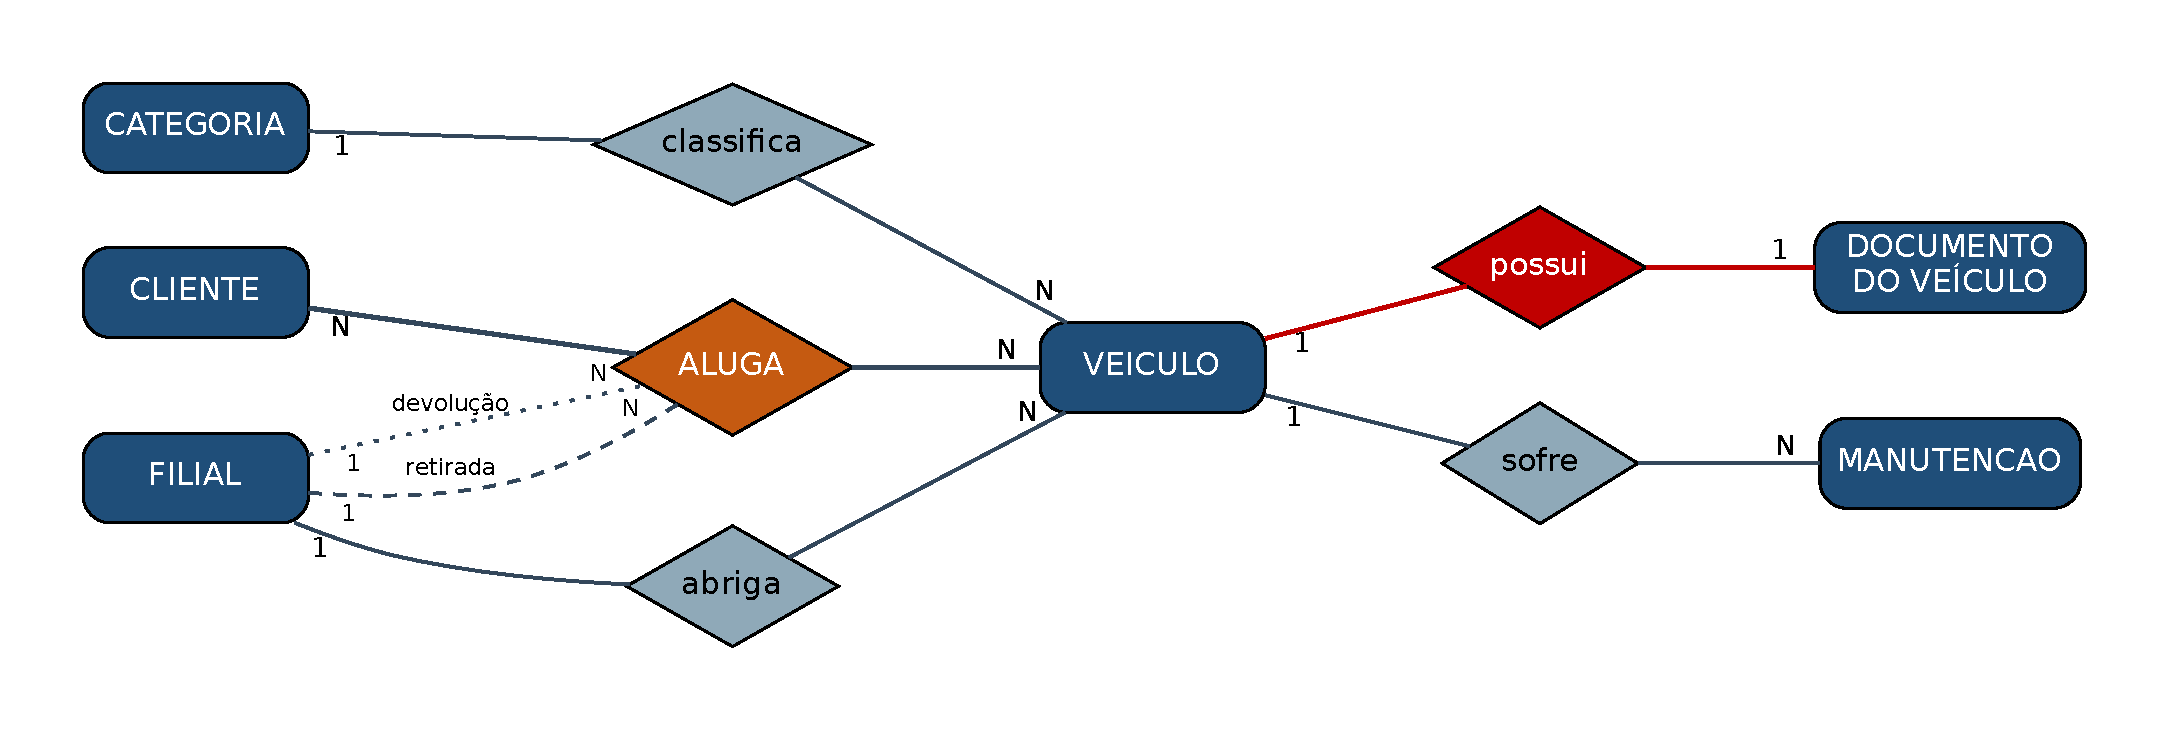
\includegraphics[width=\textwidth]{../der/der_conceitual.pdf}
\caption{Modelo conceitual do cen\'ario. O losango ALUGA, em laranja, representa o relacionamento N:N entre CLIENTE e VEICULO. Ele carrega atributos pr\'oprios (datas, quilometragens e valores) e liga-se duas vezes a FILIAL, na retirada (tracejado) e na devolu\c{c}\~ao (pontilhado). No modelo l\'ogico esse relacionamento \'e resolvido pela tabela associativa LOCACAO. O losango em vermelho representa o \'unico relacionamento 1:1 do modelo.}
\label{fig:conceitual}
\end{figure*}

\subsection{Modelo l\'ogico}

A Figura \ref{fig:der} apresenta o modelo l\'ogico completo, com as sete tabelas, os atributos, as chaves prim\'arias, as chaves estrangeiras, as restri\c{c}\~oes de unicidade e as cardinalidades de cada relacionamento.

\subsection{Cardinalidades do modelo}

O modelo cont\'em os tr\^es tipos de cardinalidade exigidos. Na Figura \ref{fig:conceitual} eles aparecem no plano conceitual e na Figura \ref{fig:der} aparecem j\'a traduzidos para chaves estrangeiras.

\begin{itemize}
\item \textbf{1:1} entre VEICULO e DOCUMENTO\_VEICULO. A chave prim\'aria de DOCUMENTO\_VEICULO \'e o pr\'oprio \texttt{id\_veiculo}, que tamb\'em \'e chave estrangeira. Com isso, cada ve\'iculo tem no m\'aximo um registro documental e nenhum registro documental existe sem ve\'iculo.
\item \textbf{1:N} em sete relacionamentos: CATEGORIA para VEICULO, FILIAL para VEICULO, CLIENTE para LOCACAO, VEICULO para LOCACAO, FILIAL para LOCACAO na retirada, FILIAL para LOCACAO na devolu\c{c}\~ao e VEICULO para MANUTENCAO.
\item \textbf{N:N} entre CLIENTE e VEICULO, resolvido pela tabela associativa LOCACAO.
\end{itemize}

\subsection{Atendimento aos pontos exigidos}

O enunciado lista quatro pontos que o modelo precisa resolver. O atendimento de cada um \'e o seguinte.

\begin{enumerate}
\item \textit{Um cliente pode ter v\'arias loca\c{c}\~oes; uma loca\c{c}\~ao pertence a um \'unico cliente.} A chave estrangeira \texttt{locacao.id\_cliente} \'e simples e obrigat\'oria, o que fixa o lado 1 em CLIENTE e o lado N em LOCACAO.
\item \textit{Um ve\'iculo pode ser alugado v\'arias vezes ao longo do tempo.} A chave prim\'aria de LOCACAO \'e \texttt{id\_locacao} e n\~ao inclui \texttt{id\_veiculo}, o que permite repetir o mesmo ve\'iculo em contratos distintos.
\item \textit{A loca\c{c}\~ao deve permitir filial de retirada e filial de devolu\c{c}\~ao diferentes.} Existem duas chaves estrangeiras independentes para FILIAL, \texttt{id\_filial\_retirada} e \texttt{id\_filial\_devolucao}, sem restri\c{c}\~ao de igualdade entre elas.
\item \textit{Cada ve\'iculo pertence a uma categoria, que define o valor da di\'aria.} O campo \texttt{valor\_diaria} fica em CATEGORIA e n\~ao em VEICULO. VEICULO guarda apenas a chave estrangeira \texttt{id\_categoria}.
\end{enumerate}

\begin{figure*}[p]
\centering
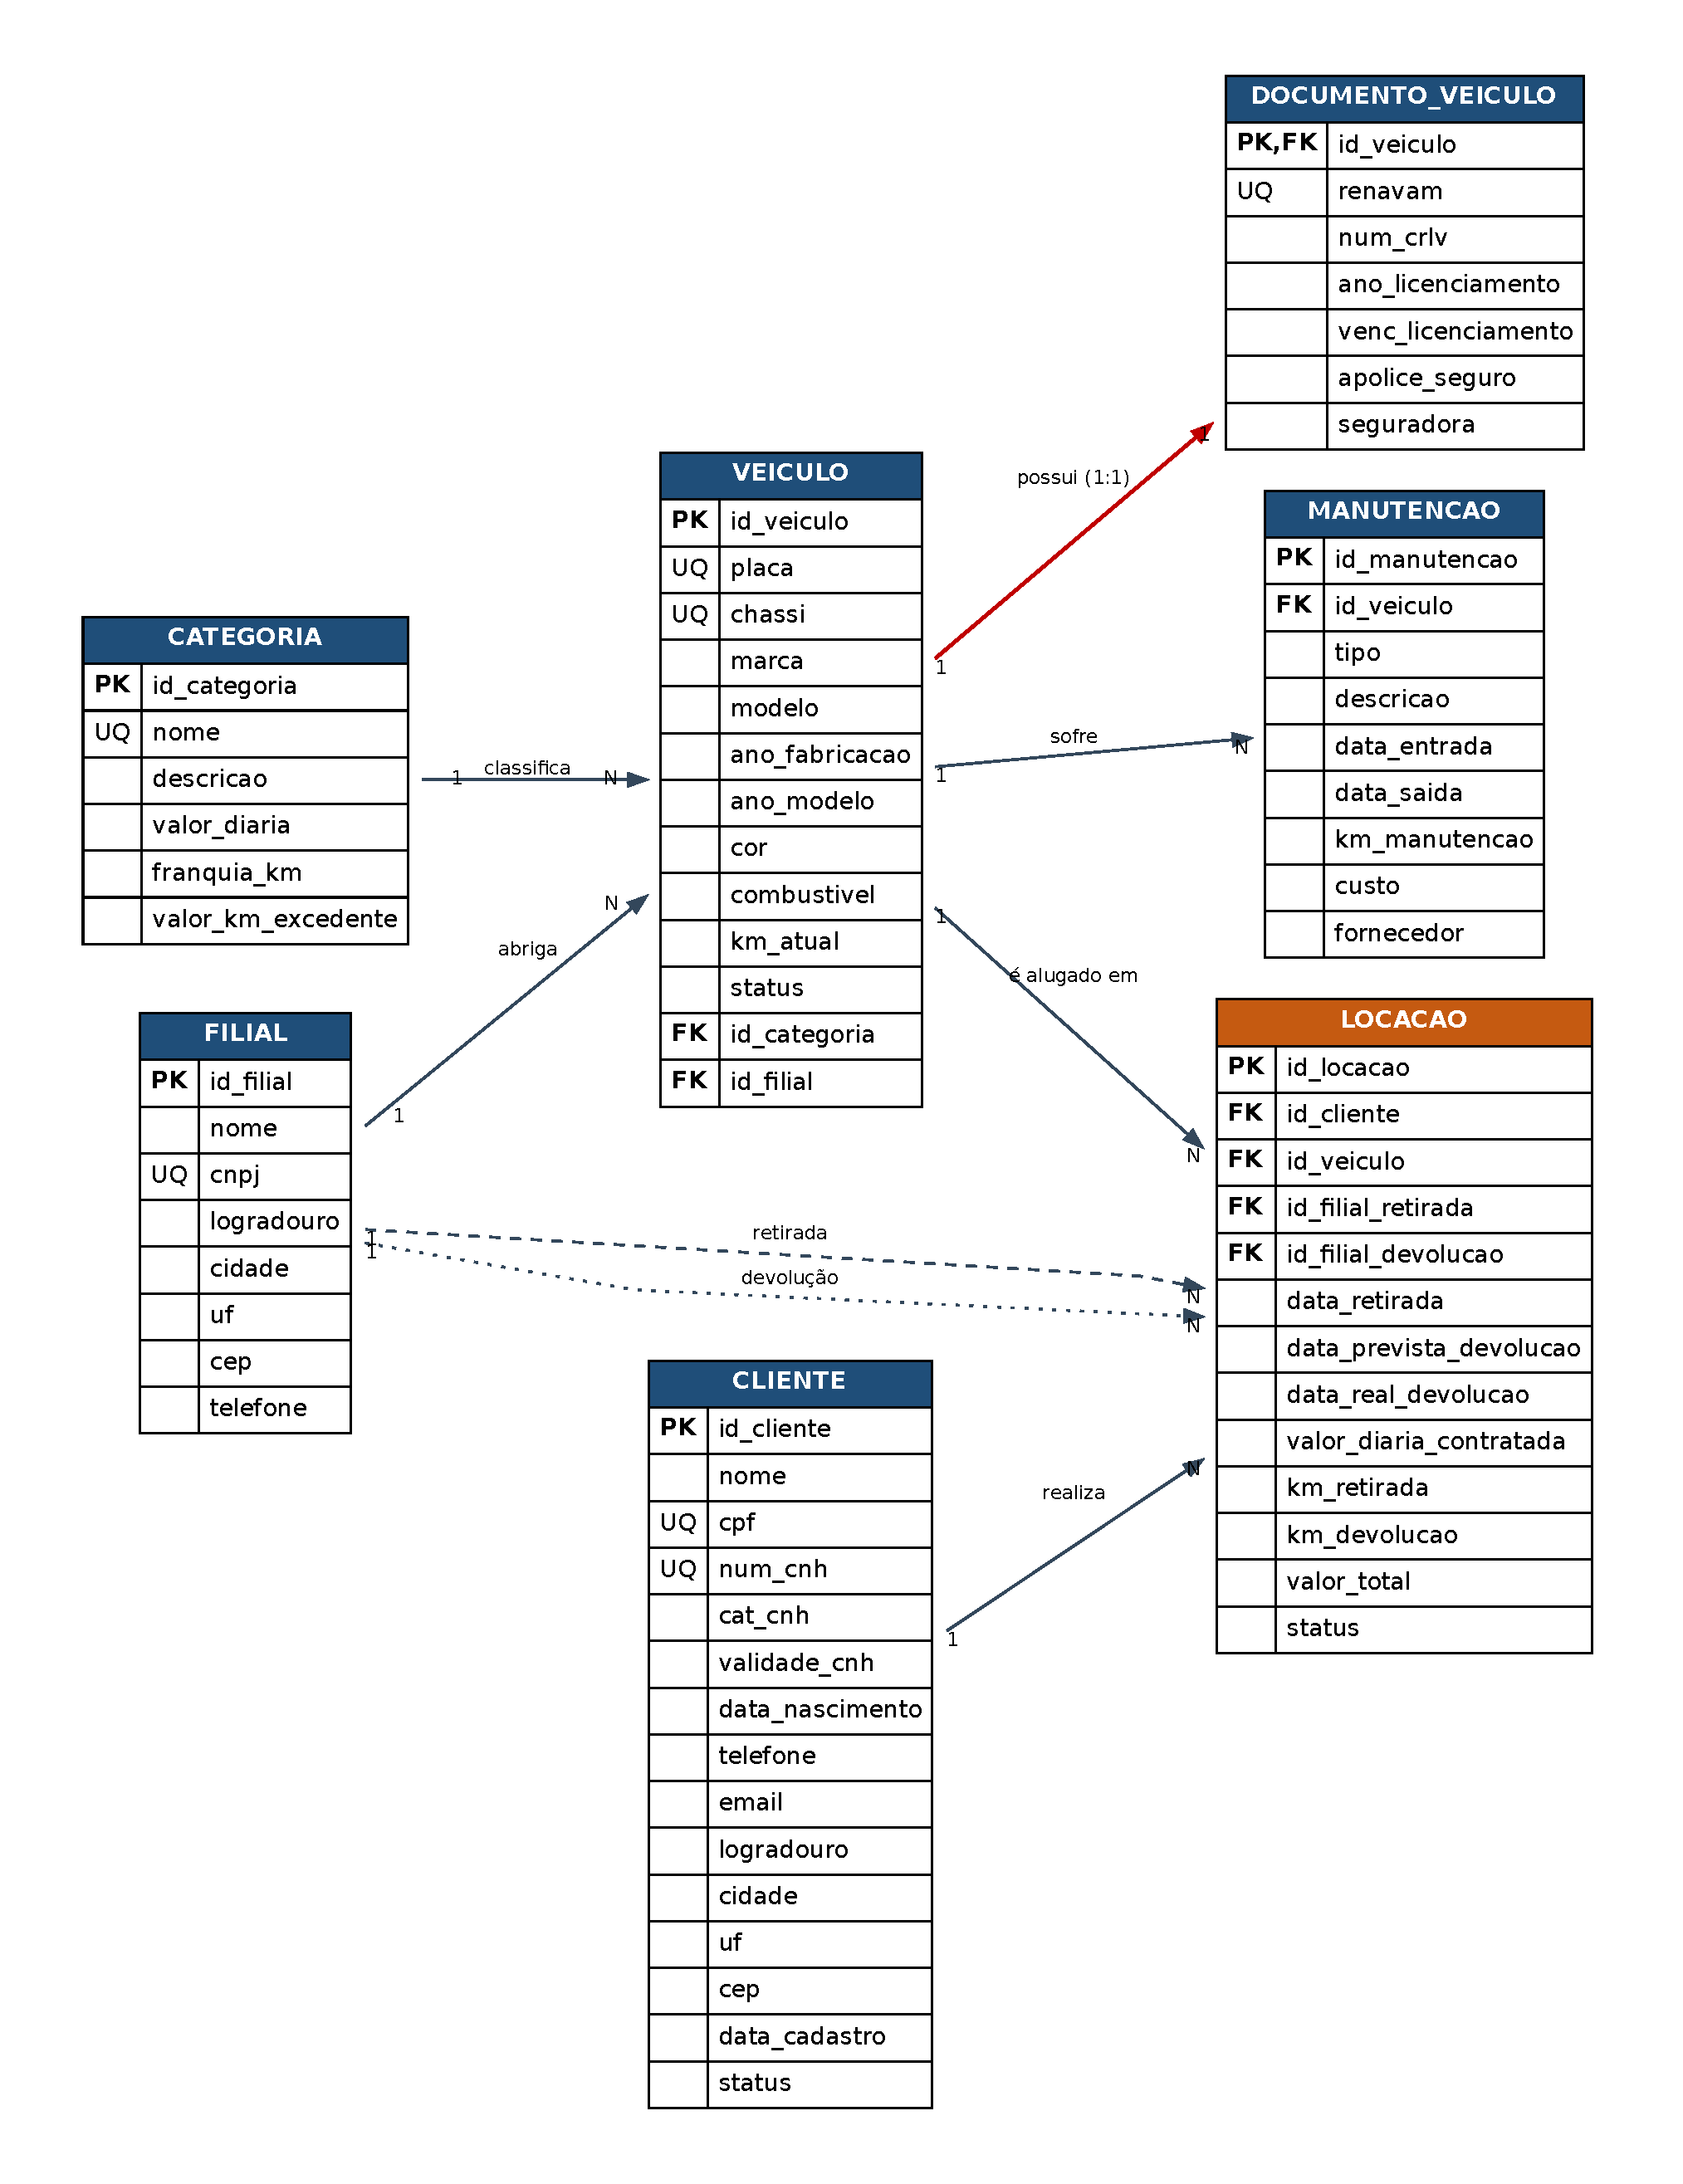
\includegraphics[height=0.92\textheight,keepaspectratio]{../der/der_logico.pdf}
\caption{Modelo l\'ogico do banco de dados da locadora, com chaves prim\'arias (PK), chaves estrangeiras (FK), restri\c{c}\~oes de unicidade (UQ) e cardinalidades. A liga\c{c}\~ao em vermelho indica o relacionamento 1:1. As liga\c{c}\~oes tracejada e pontilhada indicam, respectivamente, a filial de retirada e a filial de devolu\c{c}\~ao.}
\label{fig:der}
\end{figure*}
